% Created 2021-03-08 man 17:37
% Intended LaTeX compiler: pdflatex
\documentclass[12pt]{article}

%%%% settings when exporting code %%%% 

\usepackage{listings}
\lstdefinestyle{code-small}{
backgroundcolor=\color{white}, % background color for the code block
basicstyle=\ttfamily\small, % font used to display the code
commentstyle=\color[rgb]{0.5,0,0.5}, % color used to display comments in the code
keywordstyle=\color{black}, % color used to highlight certain words in the code
numberstyle=\ttfamily\tiny\color{gray}, % color used to display the line numbers
rulecolor=\color{black}, % color of the frame
stringstyle=\color[rgb]{0,.5,0},  % color used to display strings in the code
breakatwhitespace=false, % sets if automatic breaks should only happen at whitespace
breaklines=true, % sets automatic line breaking
columns=fullflexible,
frame=single, % adds a frame around the code (non,leftline,topline,bottomline,lines,single,shadowbox)
keepspaces=true, % % keeps spaces in text, useful for keeping indentation of code
literate={~}{$\sim$}{1}, % symbol properly display via latex
numbers=none, % where to put the line-numbers; possible values are (none, left, right)
numbersep=10pt, % how far the line-numbers are from the code
showspaces=false,
showstringspaces=false,
stepnumber=1, % the step between two line-numbers. If it's 1, each line will be numbered
tabsize=1,
xleftmargin=0cm,
emph={anova,apply,class,coef,colnames,colNames,colSums,dim,dcast,for,ggplot,head,if,ifelse,is.na,lapply,list.files,library,logLik,melt,plot,require,rowSums,sapply,setcolorder,setkey,str,summary,tapply},
aboveskip = \medskipamount, % define the space above displayed listings.
belowskip = \medskipamount, % define the space above displayed listings.
lineskip = 0pt} % specifies additional space between lines in listings
\lstset{style=code-small}
%%%% packages %%%%%

\usepackage[utf8]{inputenc}
\usepackage[T1]{fontenc}
\usepackage{lmodern}
\usepackage{textcomp}
\usepackage{color}
\usepackage{graphicx}
\usepackage{grffile}
\usepackage{wrapfig}
\usepackage{rotating}
\usepackage{longtable}
\usepackage{multirow}
\usepackage{multicol}
\usepackage{changes}
\usepackage{pdflscape}
\usepackage{geometry}
\usepackage[normalem]{ulem}
\usepackage{amssymb}
\usepackage{amsmath}
\usepackage{amsfonts}
\usepackage{dsfont}
\usepackage{array}
\usepackage{ifthen}
\usepackage{hyperref}
\usepackage{natbib}
\RequirePackage{setspace} % to modify the space between lines - incompatible with footnote in beamer
\renewcommand{\baselinestretch}{1.1}
\geometry{top=1cm}
\usepackage{titlesec}
\usepackage{etoolbox}
\makeatletter
\patchcmd{\ttlh@hang}{\parindent\z@}{\parindent\z@\leavevmode}{}{}
\patchcmd{\ttlh@hang}{\noindent}{}{}{}
\makeatother
\RequirePackage{colortbl} % arrayrulecolor to mix colors
\definecolor{myorange}{rgb}{1,0.2,0}
\definecolor{mypurple}{rgb}{0.7,0,8}
\definecolor{mycyan}{rgb}{0,0.6,0.6}
\newcommand{\lightblue}{blue!50!white}
\newcommand{\darkblue}{blue!80!black}
\newcommand{\darkgreen}{green!50!black}
\newcommand{\darkred}{red!50!black}
\definecolor{gray}{gray}{0.5}
\hypersetup{
citecolor=[rgb]{0,0.5,0},
urlcolor=[rgb]{0,0,0.5},
linkcolor=[rgb]{0,0,0.5},
}
\newenvironment{comment}{\small \color{gray}\fontfamily{lmtt}\selectfont}{\par}
\newenvironment{activity}{\color{orange}\fontfamily{qzc}\selectfont}{\par}
\RequirePackage{pifont}
\RequirePackage{relsize}
\newcommand{\Cross}{{\raisebox{-0.5ex}%
{\relsize{1.5}\ding{56}}}\hspace{1pt} }
\newcommand{\Valid}{{\raisebox{-0.5ex}%
{\relsize{1.5}\ding{52}}}\hspace{1pt} }
\newcommand{\CrossR}{ \textcolor{red}{\Cross} }
\newcommand{\ValidV}{ \textcolor{green}{\Valid} }
\usepackage{stackengine}
\usepackage{scalerel}
\newcommand\Warning[1][3ex]{%
\renewcommand\stacktype{L}%
\scaleto{\stackon[1.3pt]{\color{red}$\triangle$}{\tiny\bfseries !}}{#1}%
\xspace
}
\newcommand\Rlogo{\textbf{\textsf{R}}\xspace} %
\RequirePackage{fancyvrb}
\DefineVerbatimEnvironment{verbatim}{Verbatim}{fontsize=\small,formatcom = {\color[rgb]{0.5,0,0}}}
\RequirePackage{enumitem} % better than enumerate
\RequirePackage{epstopdf} % to be able to convert .eps to .pdf image files
\RequirePackage{capt-of} %
\RequirePackage{caption} % newlines in graphics
\RequirePackage{tikz-cd} % graph
\RequirePackage{booktabs} % for nice lines in table (e.g. toprule, bottomrule, midrule, cmidrule)
\date{\today}
\title{Univariate test vs multivariate test}
\hypersetup{
 colorlinks=true,
 pdfauthor={},
 pdftitle={Univariate test vs multivariate test},
 pdfkeywords={},
 pdfsubject={},
 pdfcreator={Emacs 27.0.50 (Org mode 9.0.4)},
 pdflang={English}
 }
\begin{document}

\maketitle
\lstset{language=r,label= ,caption= ,captionpos=b,numbers=none}
\begin{lstlisting}
library(mvtnorm)
library(data.table)
library(ggplot2)
library(ggforce) # install.packages("ggforce")
\end{lstlisting}

\section{One-dimensional test}
\label{sec:org64e92a8}

Create a 1D-grid of values corresponding to the possible values of the 1D statistic test:
\lstset{language=r,label= ,caption= ,captionpos=b,numbers=none}
\begin{lstlisting}
grid1D <- seq(-3,3,0.025)
\end{lstlisting}

The rejection region at 5\% is defined by the 0.025 and 0.975 quantiles of the normal distribution:
\lstset{language=r,label= ,caption= ,captionpos=b,numbers=none}
\begin{lstlisting}
rejection1D <- c(qnorm(0.025), qnorm(0.975))
rejection1D
\end{lstlisting}

\begin{verbatim}
[1] -1.959964  1.959964
\end{verbatim}

\lstset{language=r,label= ,caption= ,captionpos=b,numbers=none}
\begin{lstlisting}
plot(grid1D, dnorm(grid1D), type = "o", xlab = "value of the statistic test", 
     ylab = "density")
abline(v = rejection1D, col = "red")
legend("topright", col = "red", lty = 1, legend = "rejection zone", bty = "n")
\end{lstlisting}

We can then plot the values of the statistic tests and the rejection region:
\begin{center}
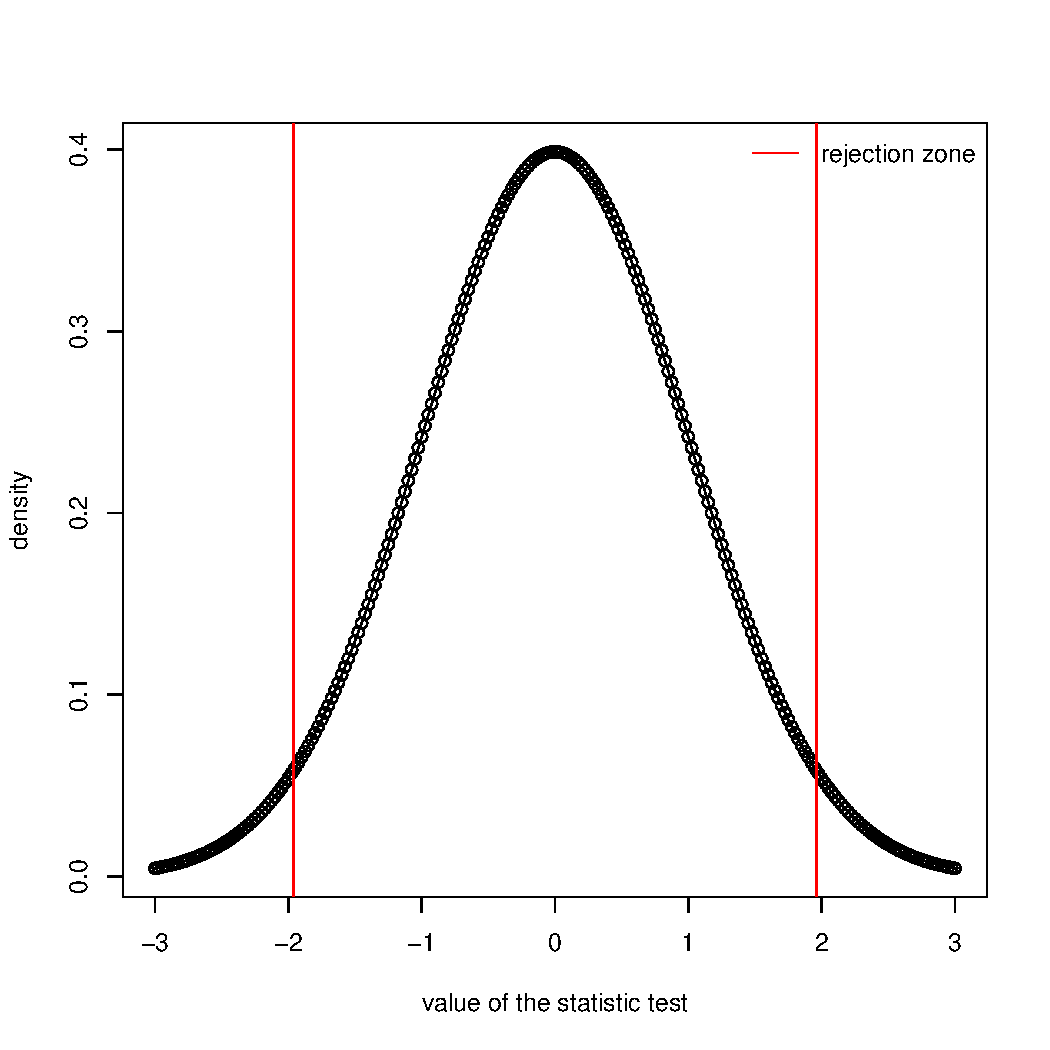
\includegraphics[width=0.7\textwidth]{figures/1D-test.pdf}
\end{center}




\section{2 dimensional test}
\label{sec:org078e43f}

Create a 2D-grid of values corresponding to the possible values of the 2D statistic test:
\lstset{language=r,label= ,caption= ,captionpos=b,numbers=none}
\begin{lstlisting}
grid2D <- as.data.table(expand.grid(beta1 = grid1D, beta2 = grid1D))
grid2D[, density := dmvnorm(cbind(beta1, beta2))]
range(grid2D$density)
\end{lstlisting}

\begin{verbatim}
[1] 1.964128e-05 1.591549e-01
\end{verbatim}

If we would do two univariate tests (not accounting for multiple
testing), the rejection region at 5\% would be a square whose size is
defined the 0.025 and 0.975 quantiles of the normal distribution:
\lstset{language=r,label= ,caption= ,captionpos=b,numbers=none}
\begin{lstlisting}
rejection2D.2uni <- data.table(xmax = qnorm(0.975, mean = 0, sd = 1),
			       ymax = qnorm(0.975, mean = 0, sd = 1),
			       xmin = qnorm(0.025, mean = 0, sd = 1),
			       ymin = qnorm(0.025, mean = 0, sd = 1))
rejection2D.2uni
\end{lstlisting}

\begin{verbatim}
       xmax     ymax      xmin      ymin
1: 1.959964 1.959964 -1.959964 -1.959964
\end{verbatim}

When we account for multiple comparison we get:
\lstset{language=r,label= ,caption= ,captionpos=b,numbers=none}
\begin{lstlisting}
qq <- qmvnorm(0.95, mean = c(0,0), sigma = diag(1,2), tail = "both")

rejection2D.2uniadj <- data.table(
    xmax = qq$quantile, ymax = qq$quantile,
    xmin = -qq$quantile,  ymin = -qq$quantile
)
rejection2D.2uniadj
\end{lstlisting}

\begin{verbatim}
       xmax     ymax      xmin      ymin
1: 2.236422 2.236422 -2.236422 -2.236422
\end{verbatim}

If we do a bivariate test, the rejection region at 5\% would be a
circle whose radius is the 0.95 quantile of a chi-squared distribution
with 2 degrees of freedom:
\lstset{language=r,label= ,caption= ,captionpos=b,numbers=none}
\begin{lstlisting}
rejection2D.chisq <- sqrt(qchisq(0.95, df = 2))
rejection2D.chisq
\end{lstlisting}

\begin{verbatim}
[1] 2.447747
\end{verbatim}

\lstset{language=r,label= ,caption= ,captionpos=b,numbers=none}
\begin{lstlisting}
gg2D <- ggplot() + labs(x=expression(beta[1]), y=expression(beta[2]))
gg2D <- gg2D + geom_raster(data = grid2D,aes(x=beta1, y=beta2, fill = density))
gg2D <- gg2D + scale_fill_gradient(low="white", high="blue")
gg2D <- gg2D + geom_rect(data = rejection2D.2uniadj, 
			 aes(xmin = xmin, xmax = xmax, ymin = ymin, ymax = ymax, 
			     colour = "2 univariate Wald tests (adjusted)"), 
			 size = 2,
			 fill  = NA) 
gg2D <- gg2D + geom_circle(aes(x0=0, y0=0, r = rejection2D.chisq, 
			       color = "1 Chi-2 test"),
			   size = 2)
gg2D <- gg2D + labs(color = "critical quantile")
gg2D
\end{lstlisting}

\begin{center}
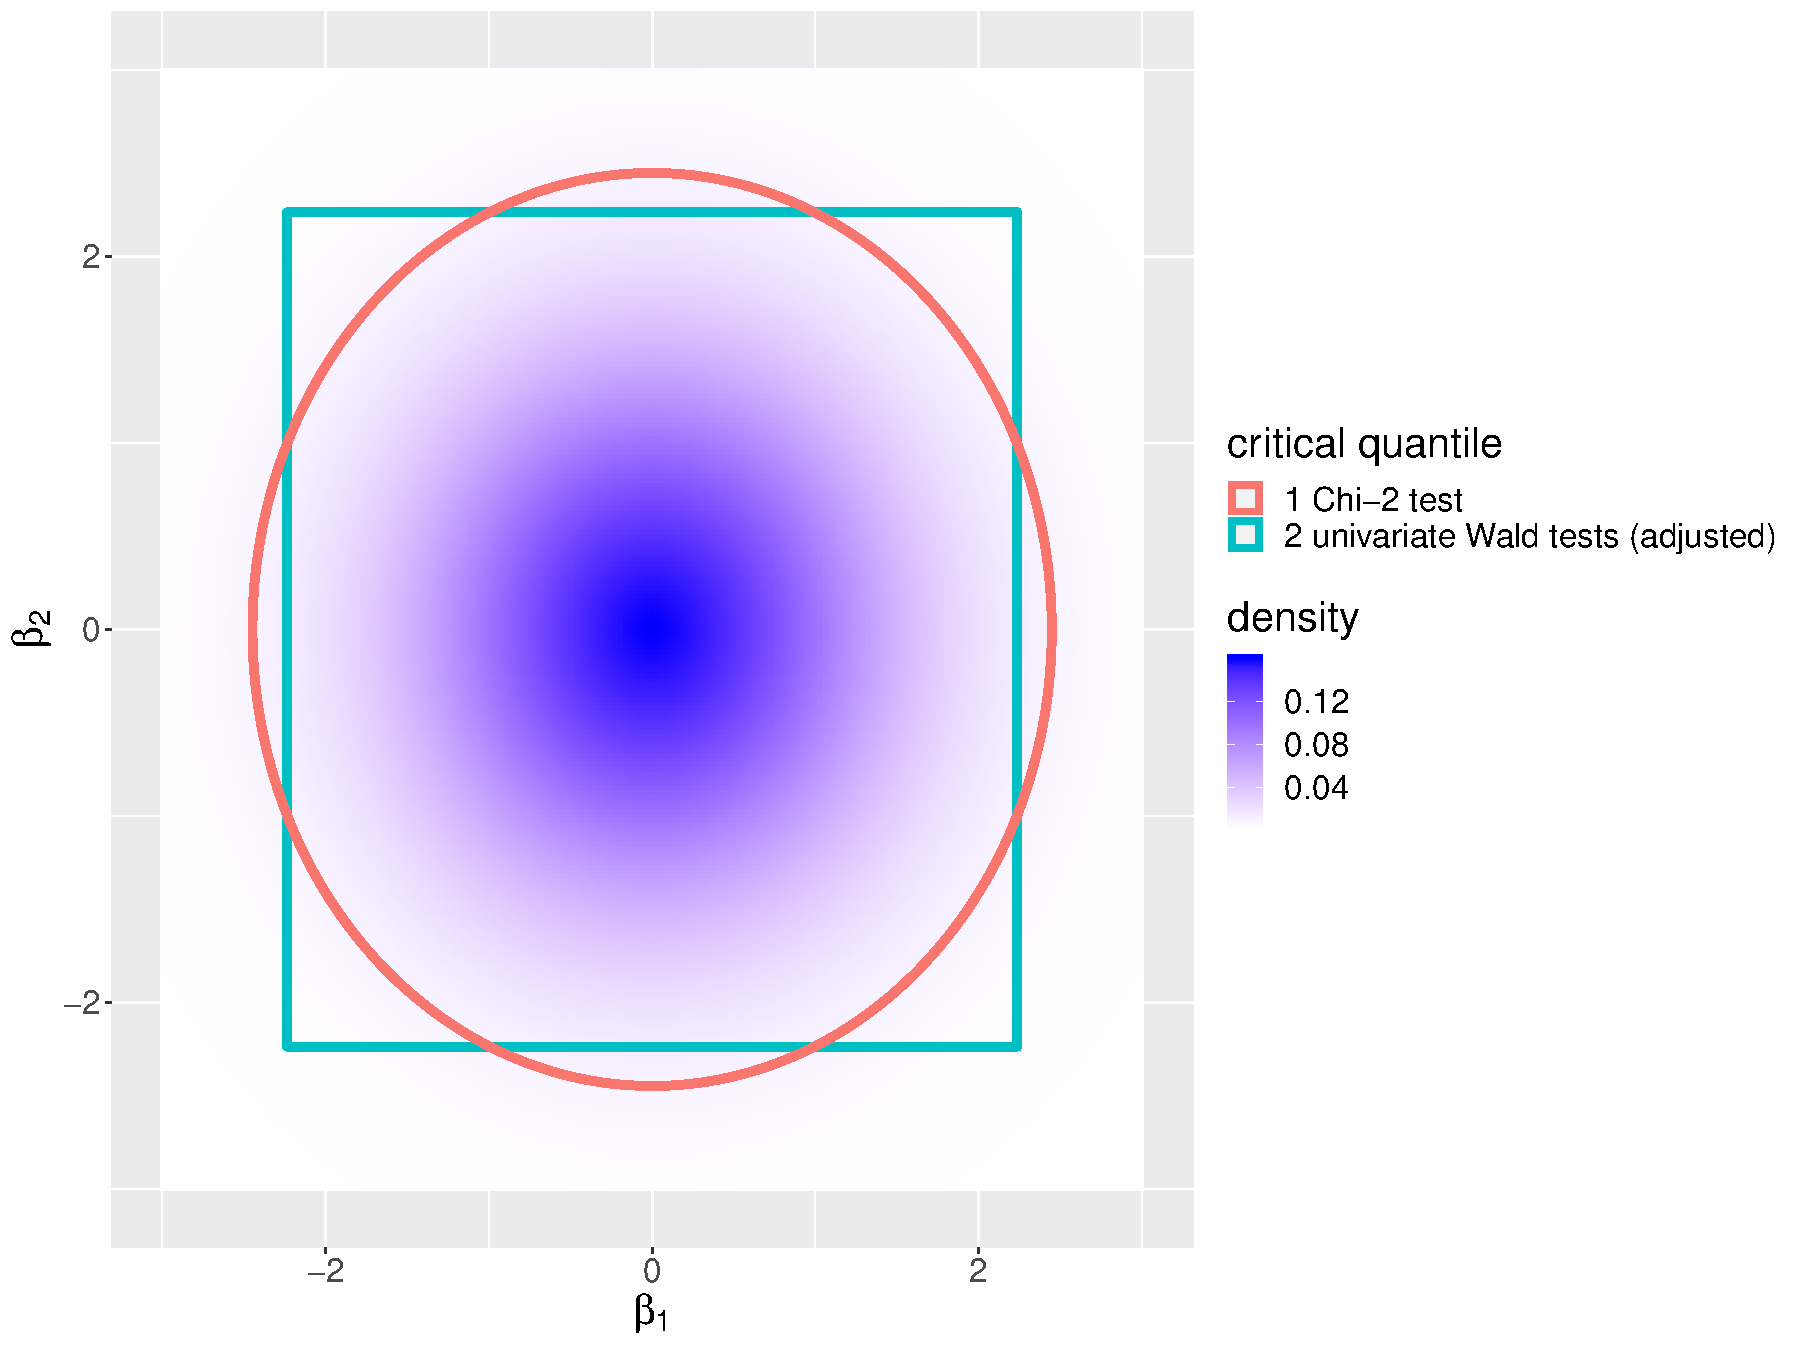
\includegraphics[width=.9\linewidth]{./figures/2D-test.pdf}
\end{center}
\end{document}